\begin{figure}[t]
\centering
\begin{subfigure}[t]{\linewidth}
\centering
\textbf{Pick Bellwether Environment}\\[0.1cm]
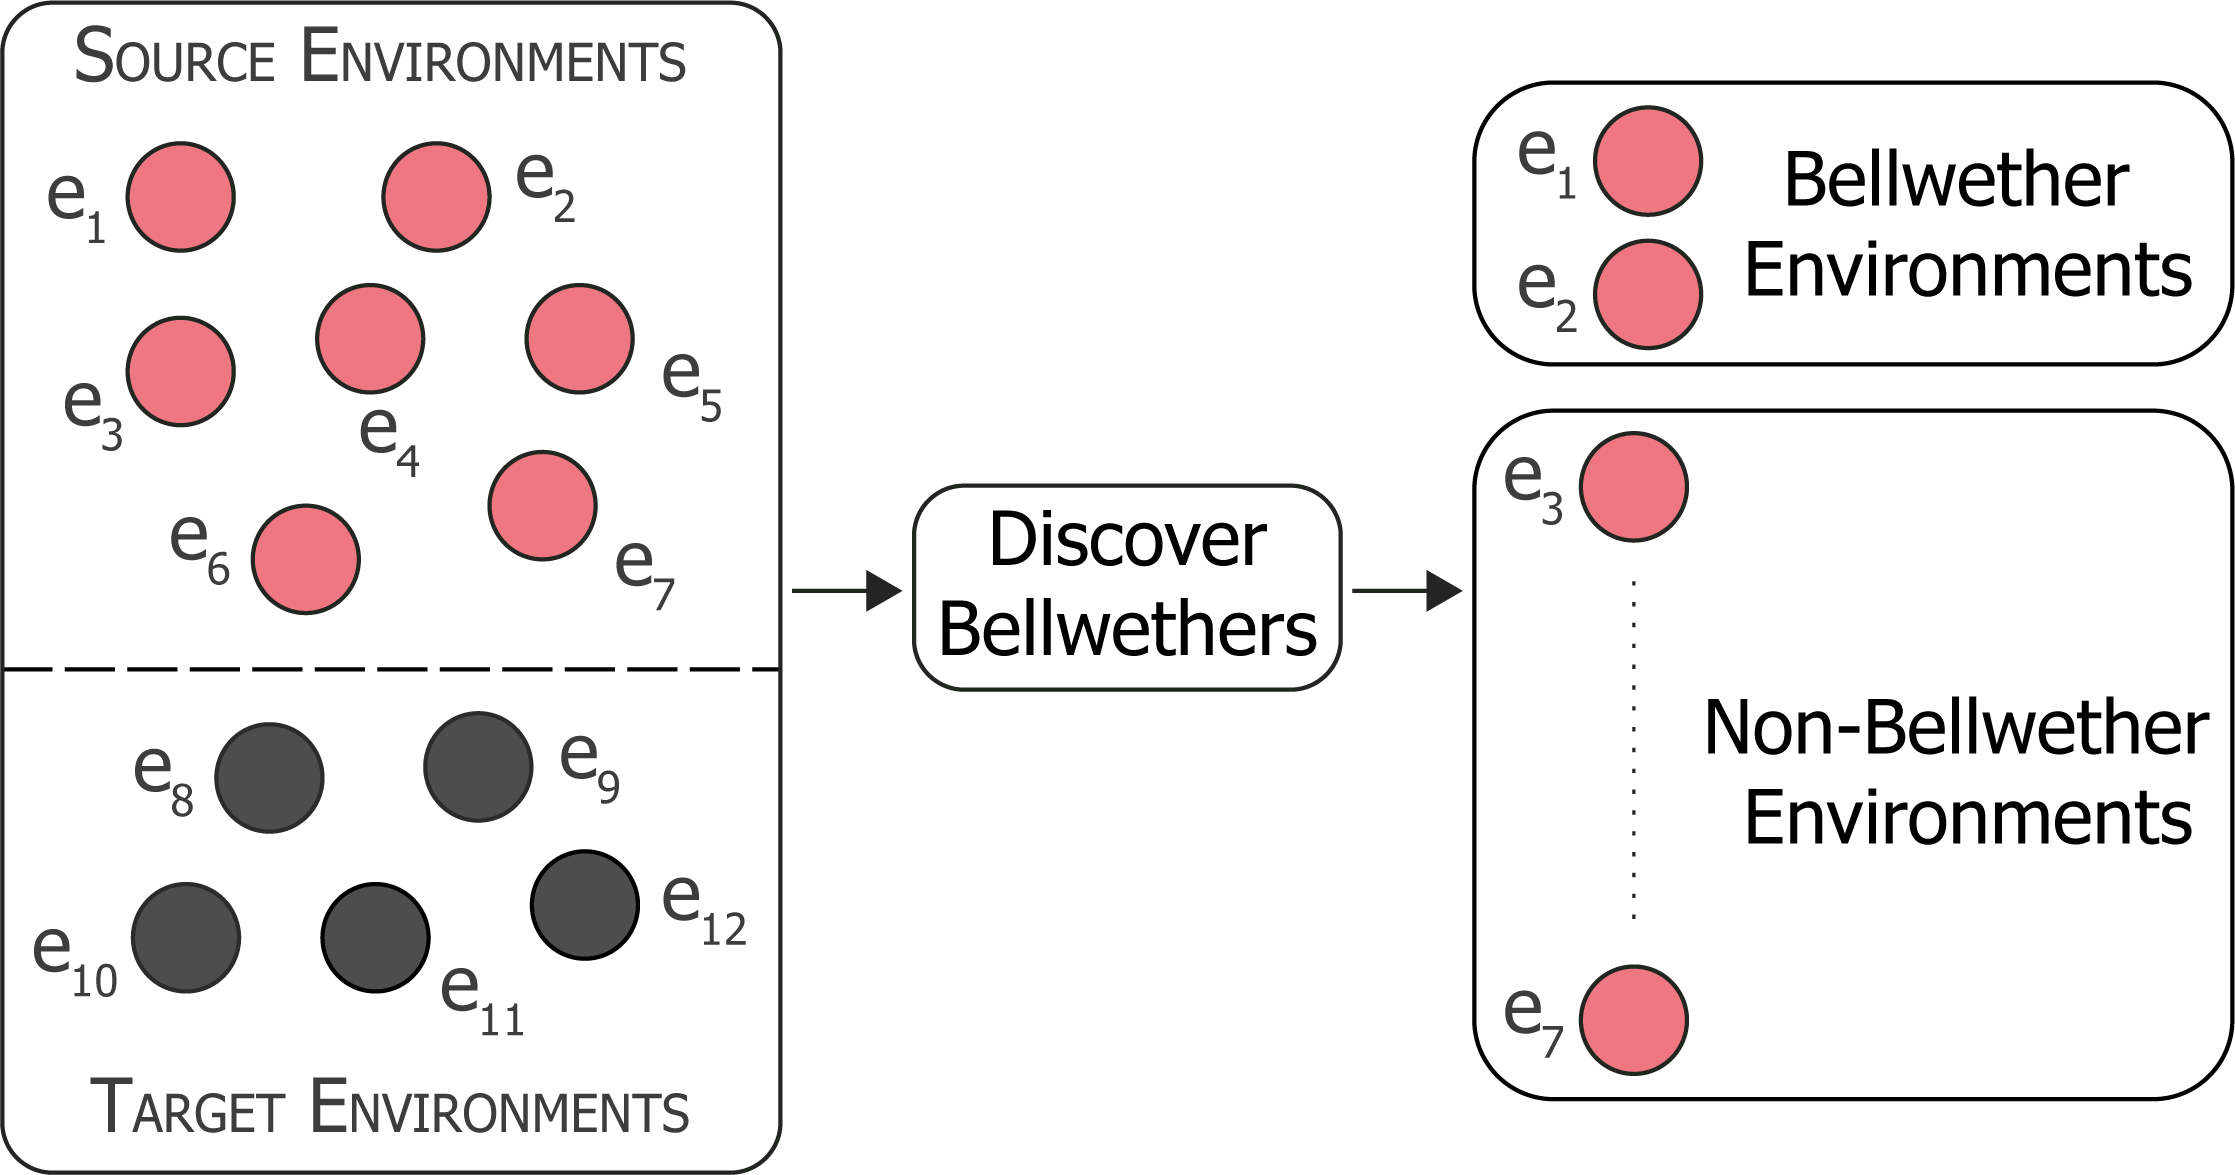
\includegraphics[width=\linewidth]{figures/source_target.png}
\end{subfigure}\\
\begin{subfigure}[t]{\linewidth}
\vspace{0.5cm}
\small
\begin{lstlisting}[xleftmargin=4.0ex,mathescape,frame=none,numbers=left]
def FindBellwether(sources, step_size, budget, thres, lives): 
  while lives or cost > budget:
   "Sample configurations"
   sampled = list()
   for source in sources:
     sampled += source.sample(step_size)
   "Get cost"
   cost = get_cost(sampled)
   "Evaluate pair-wise performances"
   perf = get_perf(sampled)
   "Remove non-bellwether environments"
   sources=remove_non_bellwethers(sources, perf, thres)
   "Loose life if no sources are removed"
   if prev == len(sources): lives -= 1
   "Return a bellwether"
  return sources[argmin(perf)]
\end{lstlisting}
\end{subfigure}
\caption{{\small This figure demonstrates how to pick the bellwethers}}
\label{fig:approach_a}
\end{figure}

\begin{figure}[t]
\begin{subfigure}[t]{\linewidth}
\centering
\textbf{Transfer Learning with Bellwether Environment}\\
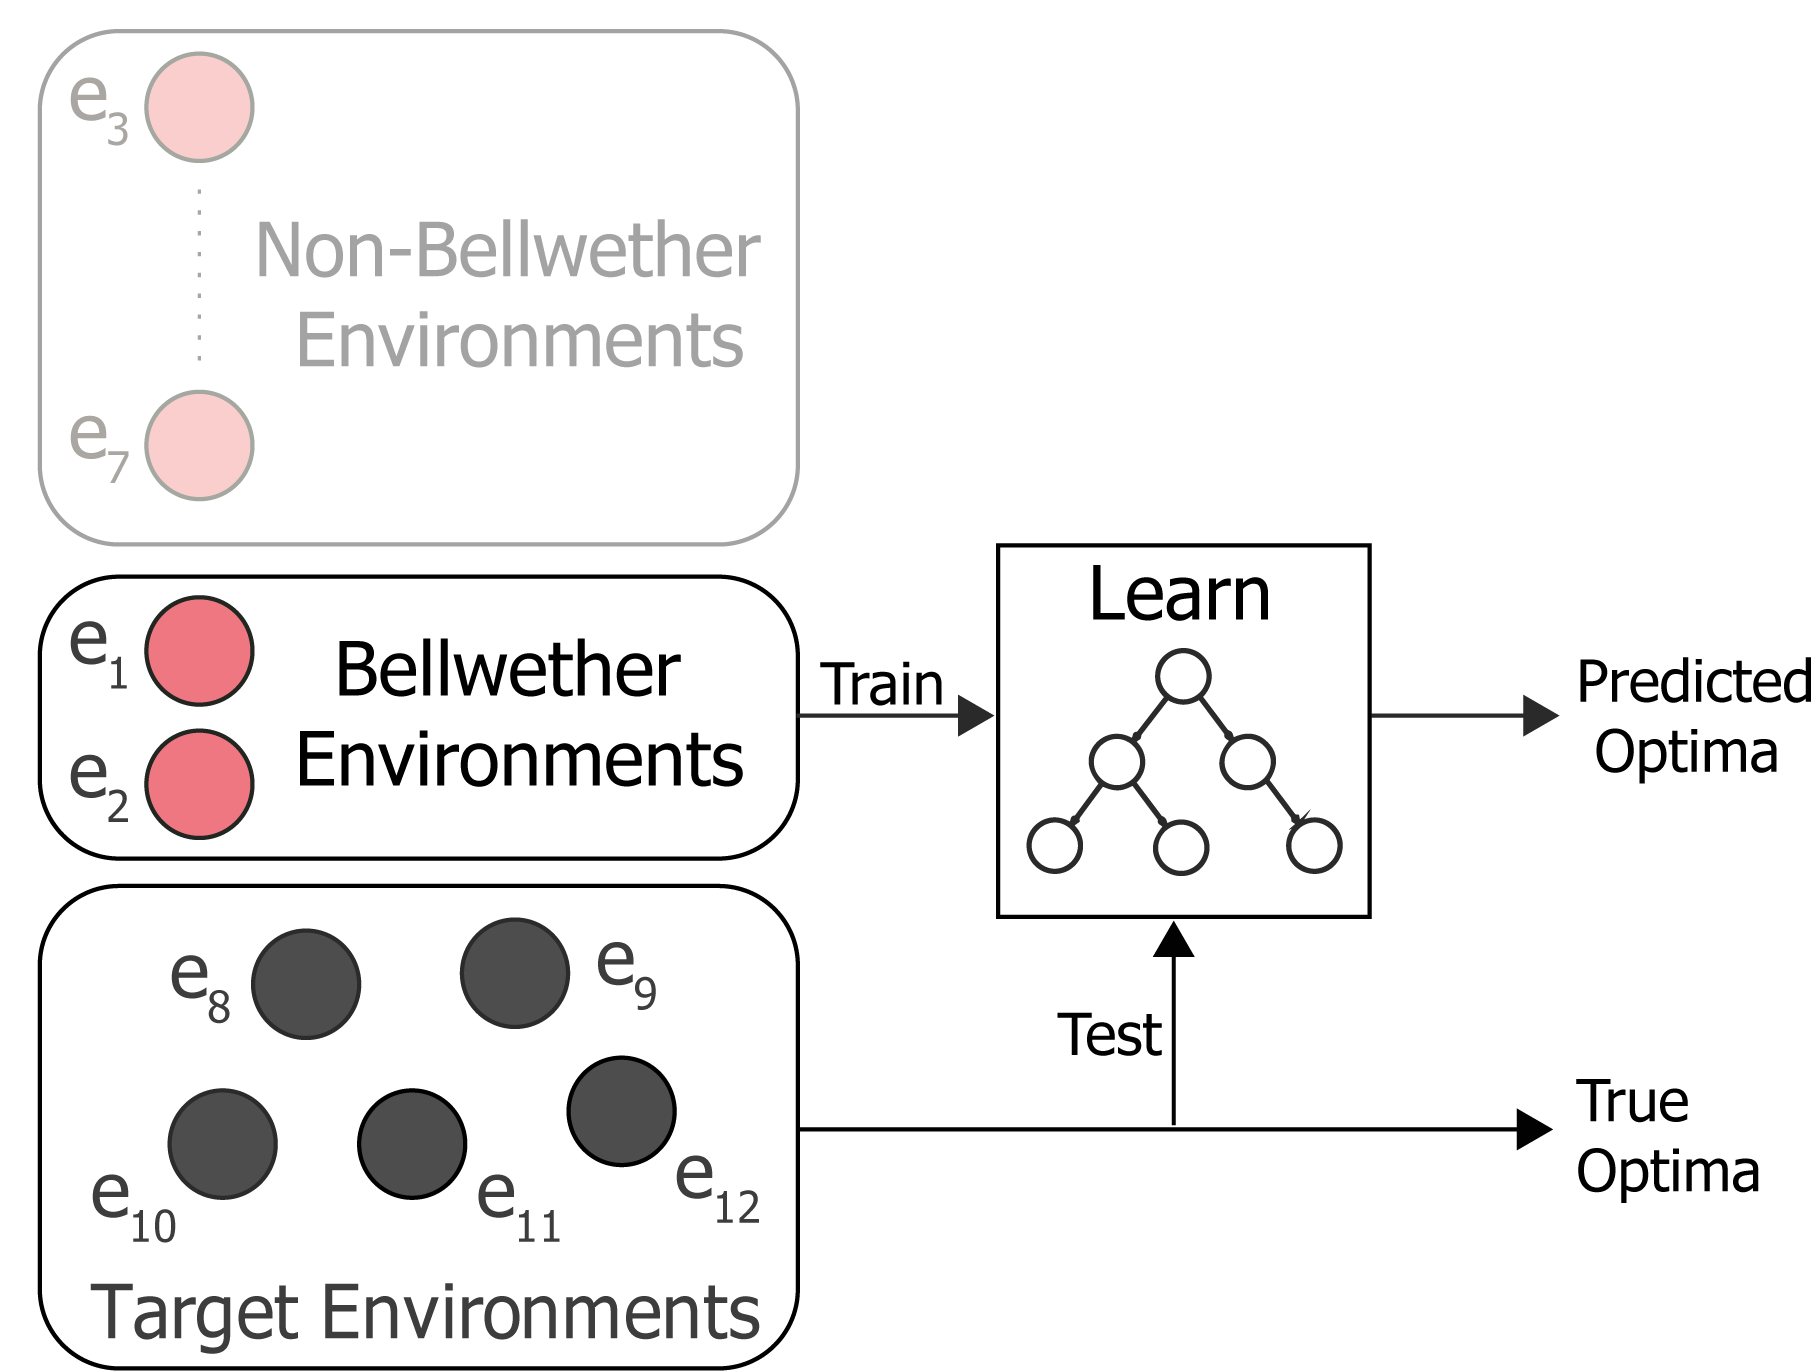
\includegraphics[width=0.85\linewidth]{figures/bellwether-transfer.png}
\end{subfigure}~~\\
\begin{subfigure}[t]{\linewidth}
\vspace{0.4cm}
\small
\begin{lstlisting}[xleftmargin=5.0ex,mathescape,frame=none,numbers=left]
def BEETLE(sources, target, budget): 
  "Find the bellwether environment"
  bellwether = FindBellwether(sources, step_size, budget, thres, lives)
  "Sample the bellwether source to fit budget"
  b_some = bellwether.sample(budget)
  "Train a prediction model with the bellwether"
  prediction_model = regTree.train(b_some)
  predicted = prediction_model.test(target.indep)
  return target[argmin(predicted)]
\end{lstlisting}
\end{subfigure}	
\caption{{\small This figure demonstrates how to construct BEETLE.}}
\label{fig:approach_b}
\end{figure}


% \begin{minipage}[]{0.475\linewidth}
% \begin{figure}
%     \centering
%     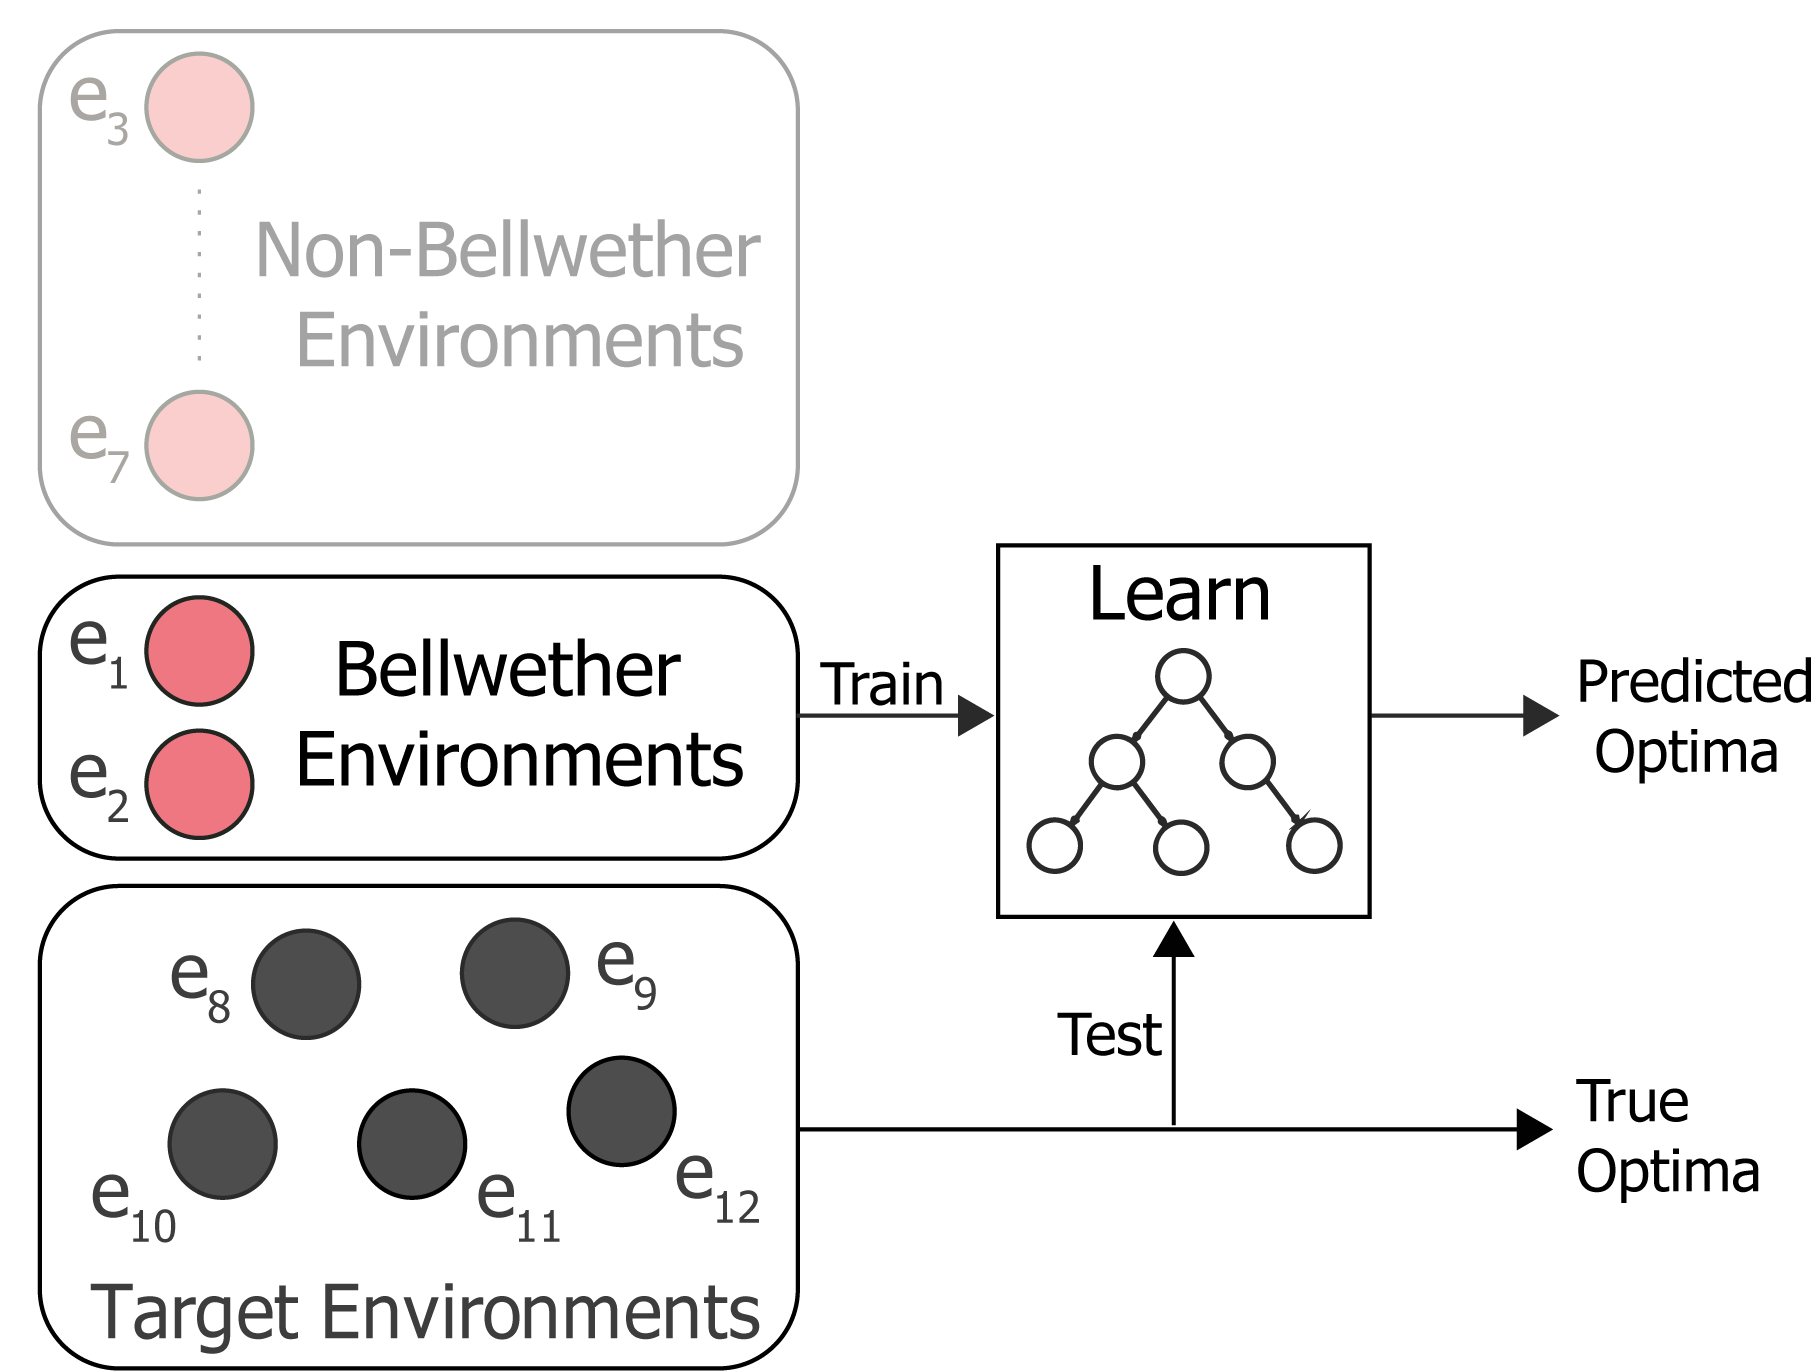
\includegraphics[width=\linewidth]{figures/bellwether-transfer.png}
% \end{figure}
% \end{minipage}\\
% \begin{minipage}[]{0.475\linewidth}

% \end{minipage}
% \begin{minipage}[]{0.475\linewidth}
% \begin{figure}[t]
% \small
% \hspace{0.2cm}\begin{lstlisting}[xleftmargin=5.0ex,mathescape,frame=none,numbers=left]
% def FindExemplar(sources, step_size, budget, lives=4): 
%   # Initializing Data Structures
%   all = model = perf = dict()
%   prev = len(sources)
%   while True:
%     # Sample new configurations and its corresponding
%     # performance measures
%     for source in sources: 
%      all[source].indep = source.sample(step_size)
%      all[source].dep = get_perf(all[source].indep)
%     for source in sources:
%      # Train a model of each source using the
%      # sampled configurations
%      model[source]=regTree()
%      model[source]=train(all[source].indep,
%                                    all[source].dep)
%      # For all the other datasets, find the performance 
%      # NAR of the model
%      for target in sources:
%       if source != target:
%          perf[source][target] = 
%               get_pairwise_perf(all[source],all[target])
%     # Find the statistics of the performance of all models
%     mean, std = get_stats(perf)
%     # Remove all the source, which performance 
%     # worse than (mean + 1*std)
%     sources = remove_not_promising(perf, (mean + std))
%     # If no sources are removed, loose life
%     if prev == len(sources): lives -= 1
%     # If total number of measurements exceed the budget, exit
%     if count(all) > budget or lives == 0: break
%   # Return the source which has the lowest performance delta 
%   return min(perf)
% \end{lstlisting}
% \end{figure}
% \end{minipage}
